\documentclass[tikz,border=4mm]{standalone}
\usetikzlibrary{positioning,fit,calc}
\tikzset{block/.style={draw,thick,text width=2cm,minimum height=1cm,align=center},
         line/.style={-latex}
     }

\begin{document}
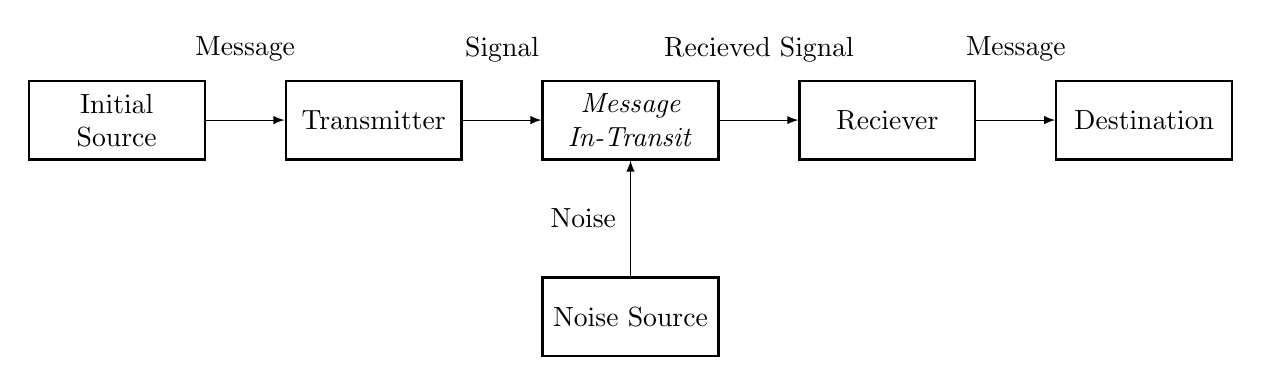
\begin{tikzpicture}
%\tikzstyle{every state}=[scale=1.2]
\node[block](a) {Initial Source};
\node[block, right=of a](b) {Transmitter};
\node[block, right=of b](c) {\textit{Message In-Transit}};
\node[block, right=of c](d) {Reciever};
\node[block, right=of d](e) {Destination};
\node[block] (f) at ([yshift=-2.5cm]$(b)!1.0!(c)$) {Noise Source};
\draw[line] (a)-- node[yshift=+0.9cm] {Message} (b);
\draw[line] (b)-- node[yshift=+0.9cm] {Signal} (c);
\draw[line] (c)-- node[yshift=+0.9cm] {Recieved Signal} (d);
\draw[line] (d)-- node[yshift=+0.9cm] {Message} (e);
\draw[line] (f)-- node[xshift=-0.6cm] {Noise} (c);
\end{tikzpicture}
\end{document}
